\newpage
\section{Resultados}

\subsection{Rede $L$}

Foram calculados os parâmetros dos componentes da rede L conforme o procedimento descrito na seção \ref{subsec:l}, chegando-se no circuito mostrado na figura \ref{f_sch_rede_L}.

\begin{figure}[H]
    \centering
    \caption{Circuito da rede L.}
    \includegraphics[scale=0.5]{Imagens/ex1/sch.png}
    \label{f_sch_rede_L}
    
    \small Fonte: Autoria própria.
\end{figure}

As formas de onda no domínio do tempo obtidas para o circuito são mostradas na figura \ref{fig:ondas}.

\begin{figure}[H]
    \centering
    \caption{Formas de onda na fonte, entrada da rede L e sobre a carga.}
    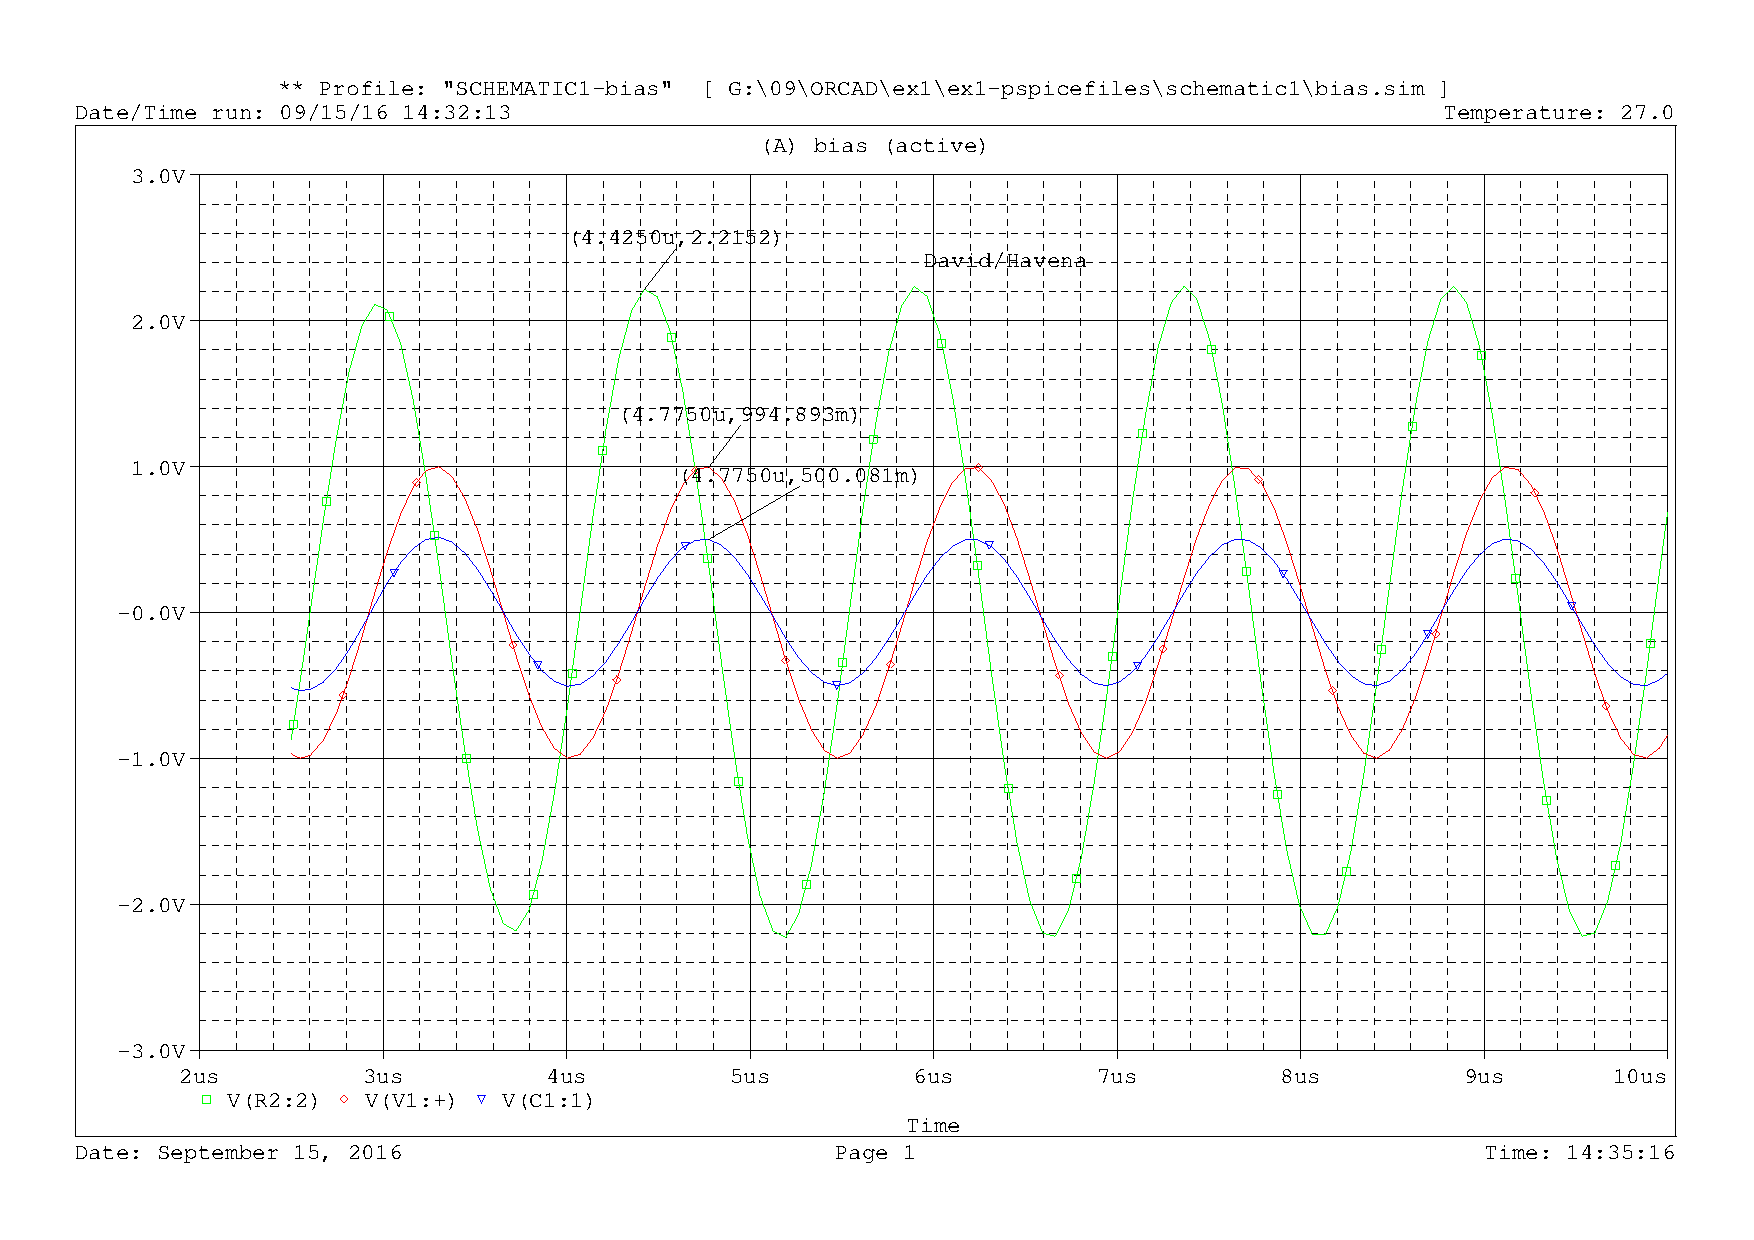
\includegraphics[scale=0.5]{Imagens/ex1/ondas.pdf}
    \label{fig:ondas}
    
    \small Fonte: Autoria própria.
\end{figure}

O circuito foi então simulado no modo AC-Sweep, onde foi obtido o gráfico da magnitude da resposta em frequência, mostrado na figura \ref{f_rede_L_graph}.

\begin{figure}[H]
    \centering
    \caption{Resposta em frequência da rede L.}
    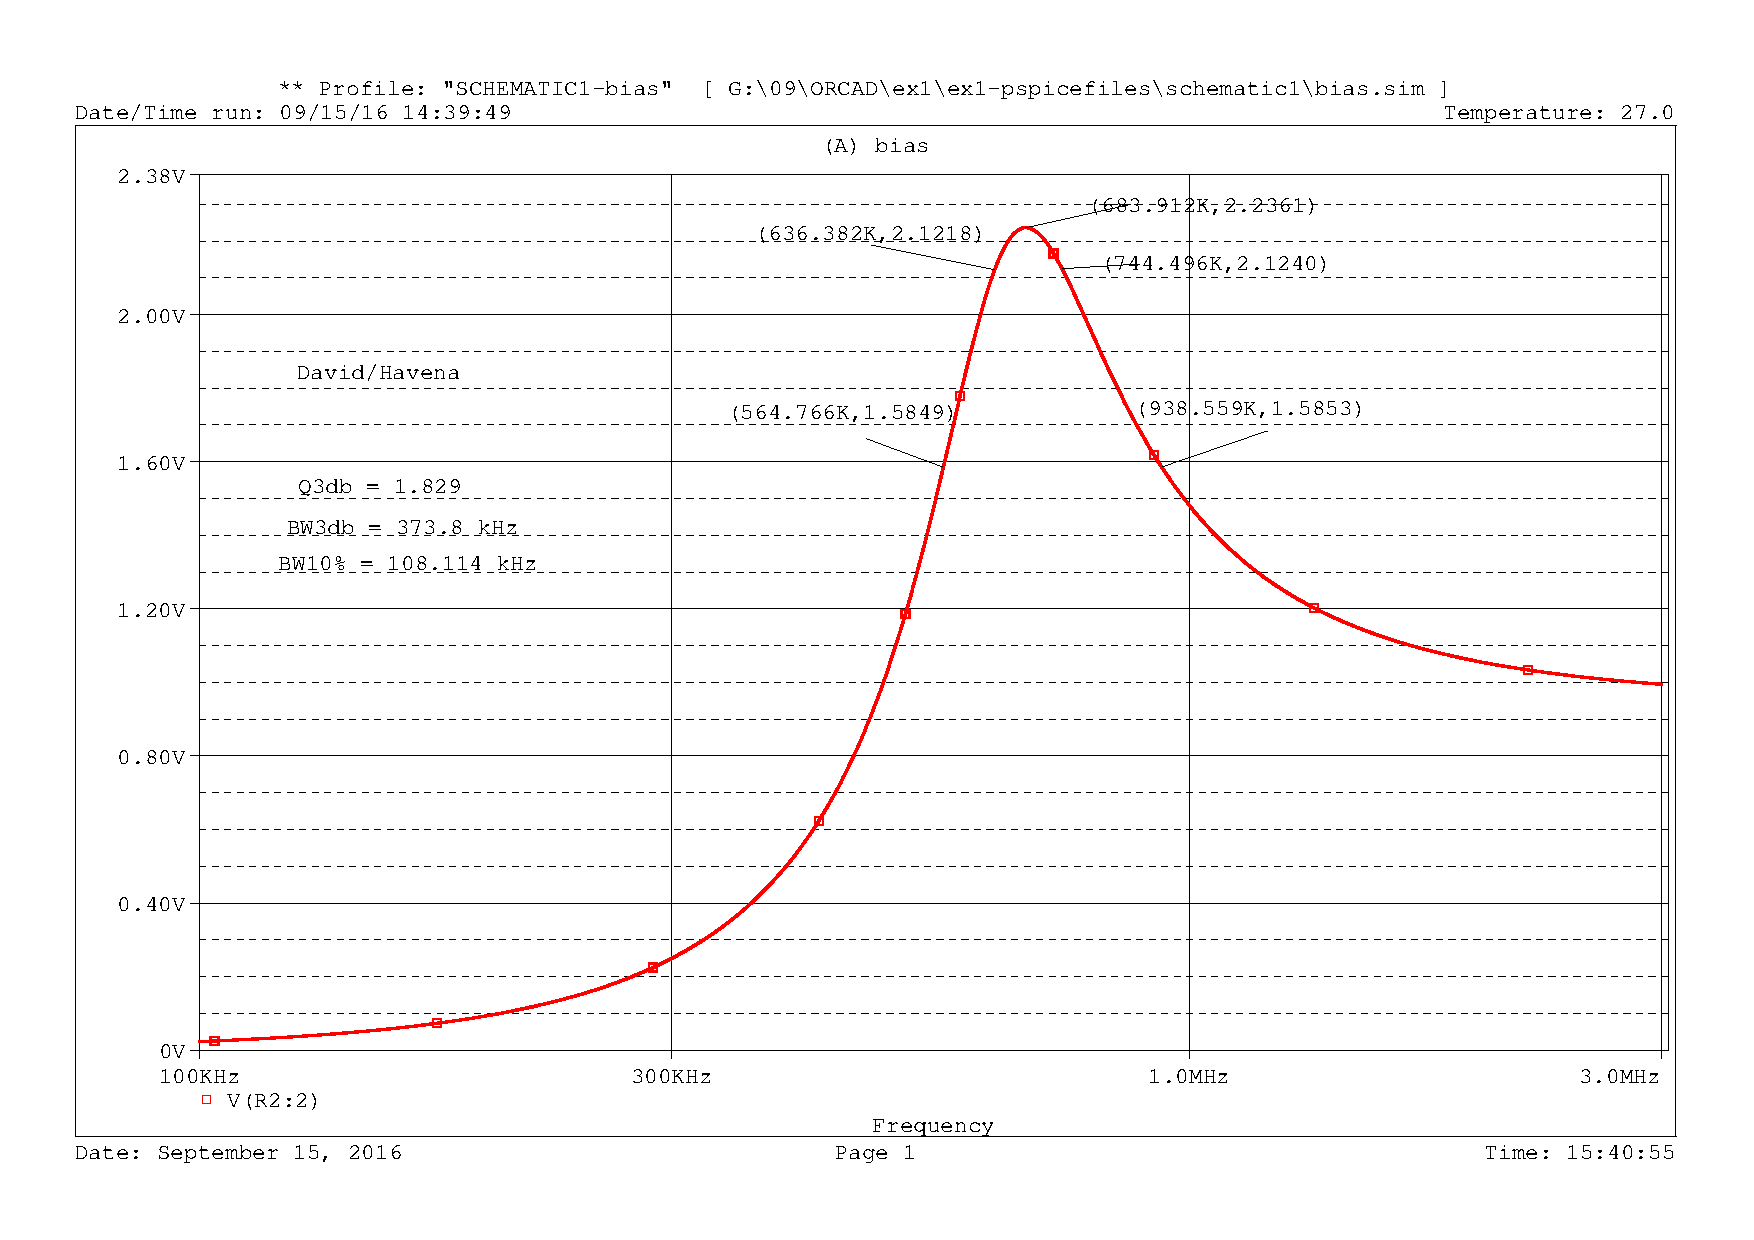
\includegraphics[scale=0.5]{Imagens/ex1/resf.pdf}
    \label{f_rede_L_graph}
    
    \small Fonte: Autoria própria.
\end{figure}

Os dados obtidos com o experimento estão descriminados na tabela \ref{tab:resl}.

\begin{table}[H]
    \centering
    \caption{Resultados para rede L.}
    \label{tab:resl}
    \begin{tabular}{cccc}
     \hline
     $f_c$ & $BW_{3dB}$ & $BW_{pot}$ & $Q$ \\
     \hline
      683,912 kHz & 373,8kHz & 108,114 kHz & 1,829 \\
     \hline
    \end{tabular}

    \small Fonte: Autoria própria.
\end{table}

Sendo $f_c$ a frequência central, $BW_{3dB}$ a banda de 3dB, $BW_{pot}$ a banda pelo critério da potência e $Q$ o fator de mérito.

Observa-se que pelo critério da potência, a largura de banda é mais estreita do que pelo critério de 3dB.
 
\subsection{Rede $T$}
 
Para o segundo experimento a rede T foi escolhida, sendo calculados os parâmetros dos componentes da rede, mostrado na figura \ref{f_sch_rede_T}.
 
\begin{figure}[H]
    \centering
    \caption{Circuito da rede T.}
    \includegraphics[scale=0.7]{Imagens/ex3/sch.png}
    \label{f_sch_rede_T}
    
    \small Fonte: Autoria própria.
\end{figure}
    
O circuito foi então simulado no modo AC-Sweep, onde foi obtido o gráfico da figura \ref{f_rede_T_graph}.
    
\begin{figure}[H]
    \centering
    \caption{Módulo da resposta em frequência para rede T.}
    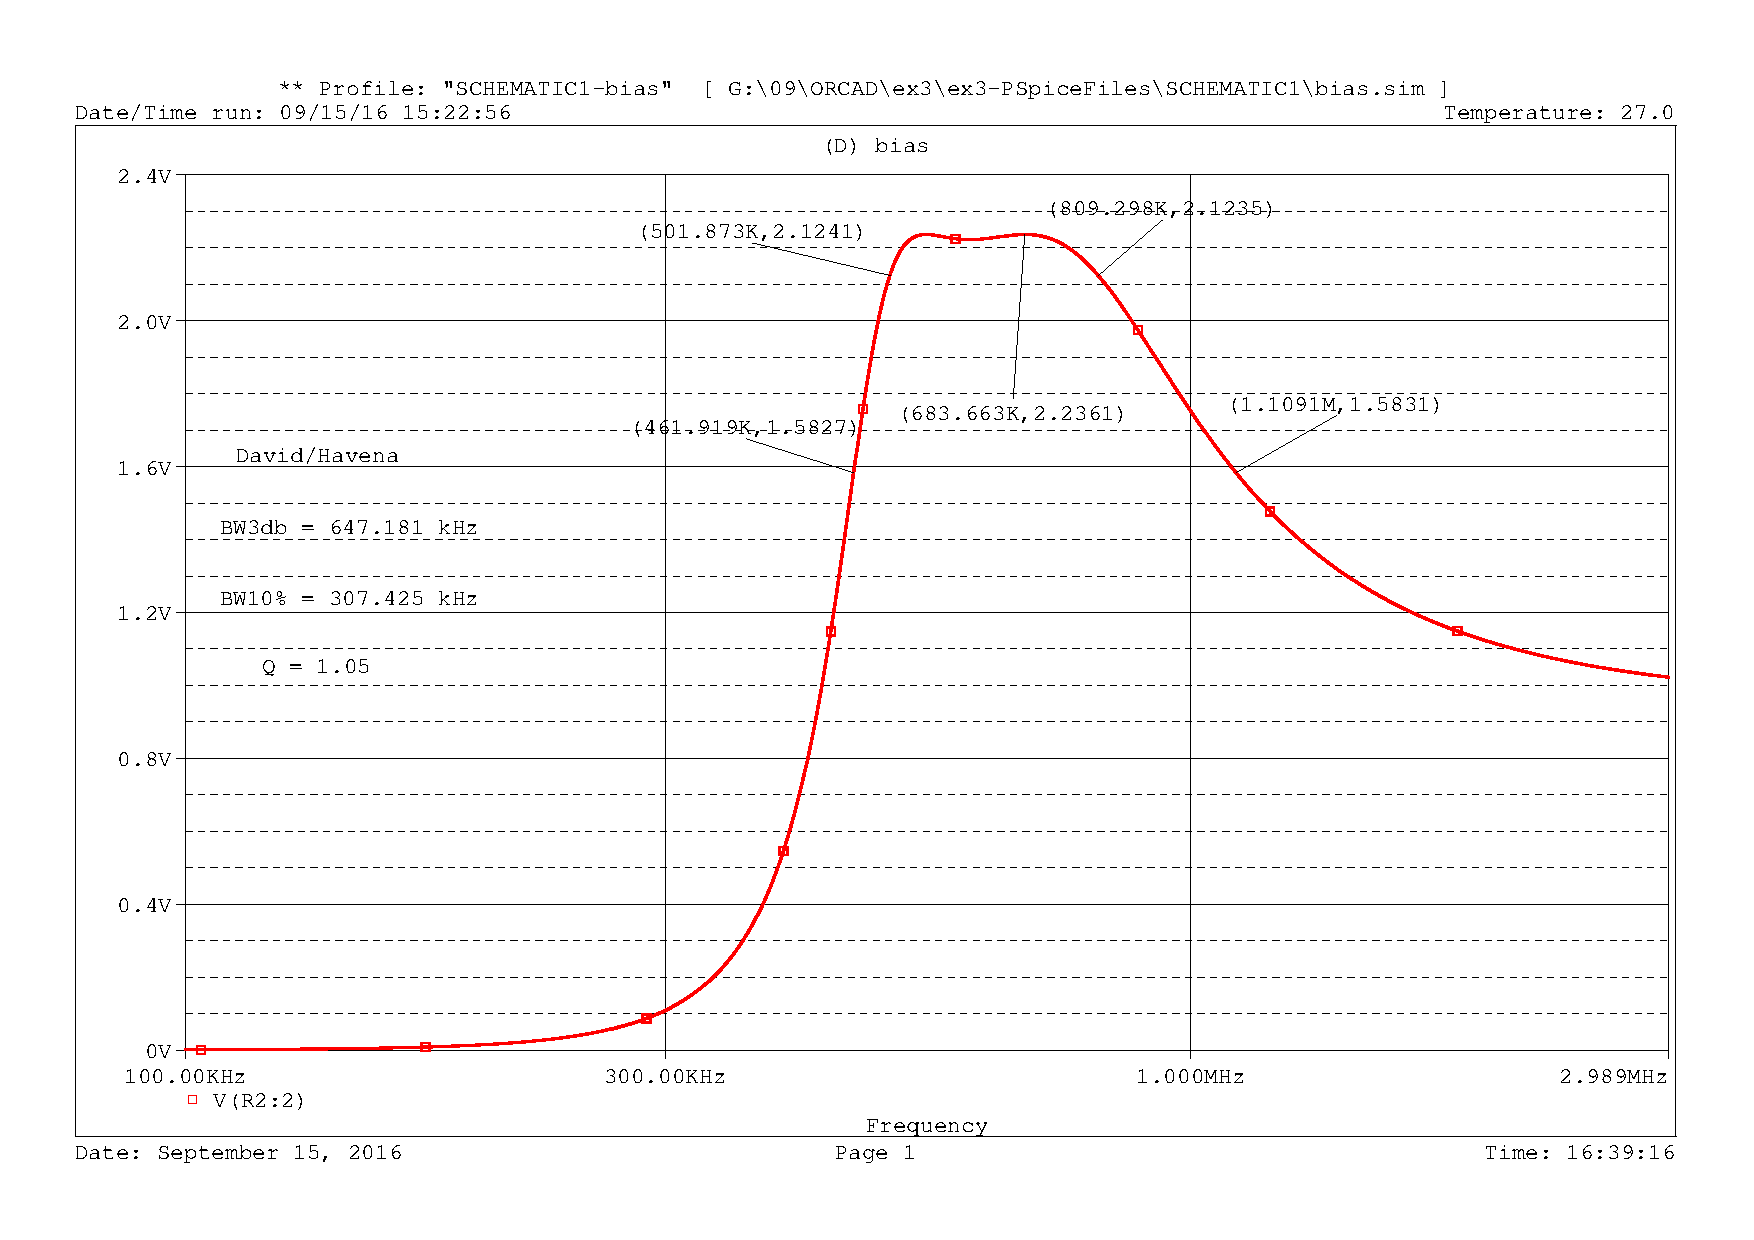
\includegraphics[scale=0.5]{Imagens/ex3/fres.pdf}
    \label{f_rede_T_graph}
    
    \small Fonte: Autoria própria.
\end{figure}
    
Os dados obtidos com o experimento estão descriminados na tabela \ref{tab:rest}.

\begin{table}[H]
    \centering
    \caption{Resultados para rede T.}
    \label{tab:rest}
    \begin{tabular}{cccc}
        \hline
        $f_c$ & $BW_{3dB}$ & $BW_{pot}$ & $Q$ \\
        \hline
        683,912 kHz & 330,8kHz & 109,84 kHz & 2,067 \\
        \hline
    \end{tabular}
    
    \small Fonte: Autoria própria.
\end{table}

\subsection{Rede $L_{wideband}$}

Foram calculados os parâmetros dos componentes da rede $L_{wideband}$, chegando-se no circuito mostrado na figura \ref{f_sch_rede_L_wideband}.

\begin{figure}[H]
    \centering
    \caption{Circuito da rede $L_{wideband}$.}
    \includegraphics[scale=0.7]{Imagens/ex2/sch.png}
    \label{f_sch_rede_L_wideband}
    
    \small Fonte: Autoria própria.
\end{figure}

De modo a reduzir o número de componentes no circuito, os dois capacitores em paralelo foram substituídos por um único capacitor equivalente, como mostra a figura \ref{fig:sch2}.

\begin{figure}[H]
    \centering
    \caption{Circuito da rede $L_{wideband}$.}
    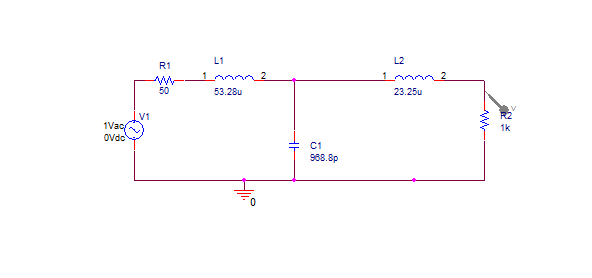
\includegraphics[scale=0.7]{Imagens/ex2/sch2.png}
    \label{fig:sch2}
    
    \small Fonte: Autoria própria.
\end{figure}  

O circuito foi então simulado no modo AC-Sweep, onde foi obtido o gráfico da figura \ref{f_rede_L_wideband_graph}.

\begin{figure}[H]
    \centering
    \caption{Módulo da resposta em frequência da rede $L_{wideband}$L.}
    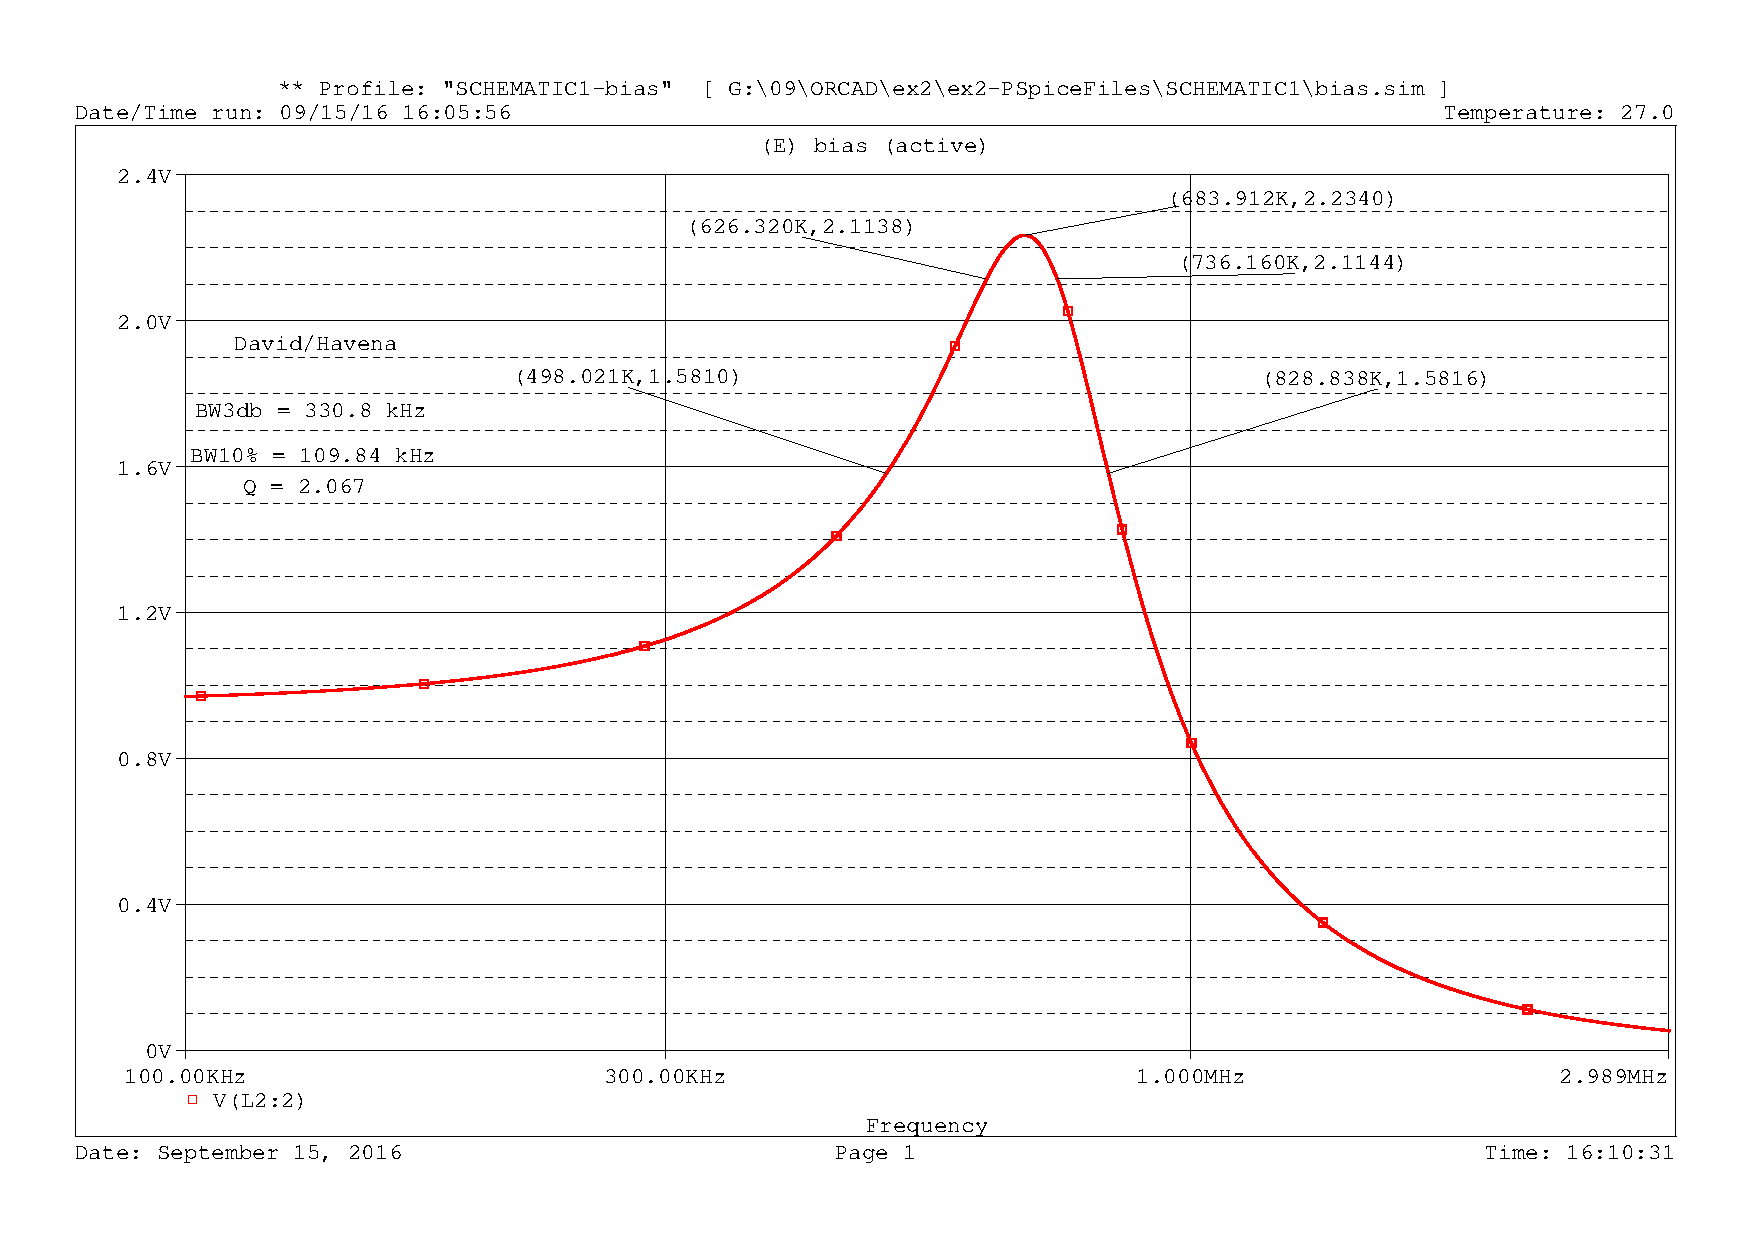
\includegraphics[scale=0.5]{Imagens/ex2/fres.pdf}
    \label{f_rede_L_wideband_graph}
    
    \small Fonte: Autoria própria.
\end{figure}

Os dados obtidos com o experimento estão descriminados na tabela \ref{tab:reslwb}.

\begin{table}[H]
    \centering
    \caption{Resultados para rede $L_{wideband}$.}
    \label{tab:reslwb}
    \begin{tabular}{cccc}
        \hline
        $f_c$ & $BW_{3dB}$ & $BW_{pot}$ & $Q$ \\
        \hline
        683,663 kHz & 647,181kHz & 307,425 kHz & 1,05 \\
        \hline
    \end{tabular}
    
    \small Fonte: Autoria própria.
\end{table}

Observa-se que a adição de uma segunda camada a rede L aumentou consideravelmente a largura de banda.
